\documentclass[11pt]{article}
\usepackage[margin=1in]{geometry}
\usepackage{amsmath,amssymb,amsthm}
\usepackage{graphicx}
\usepackage[hidelinks]{hyperref}

\newtheorem*{theorem}{Theorem}

\title{Literature Status for Problem 14 of arXiv:1207.2958}
\author{FA/Banach run packet}
\date{June 14, 2026}

\begin{document}
\maketitle

\section*{Status}

\textbf{Result type:} literature already answered.

\textbf{Source problem:} Godefroy--Lancien--Zizler, \emph{The non-linear
geometry of Banach spaces after Nigel Kalton}, arXiv:1207.2958, Problem 14.

\textbf{Supporting answer:} Baudier--Lancien--Schlumprecht, \emph{The coarse
geometry of Tsirelson's space and applications}, arXiv:1705.06797.

\section*{Open Problem Evidence}

The source survey asks the following question in Problem 14.

\begin{center}

\includegraphics[width=\linewidth]{figures/open_problem_crop.png}
\end{center}

Transcription:
\[
\text{Does }\ell_2\text{ coarsely embed into every infinite dimensional Banach space?}
\]

The word ``infinite'' is part of the source statement. This packet is therefore
not based on a finite-dimensional reading.

\section*{Supporting Literature Evidence}

The later paper explicitly identifies the same question as Problem 14 in the
survey and restates it as the Main Problem.

\begin{center}
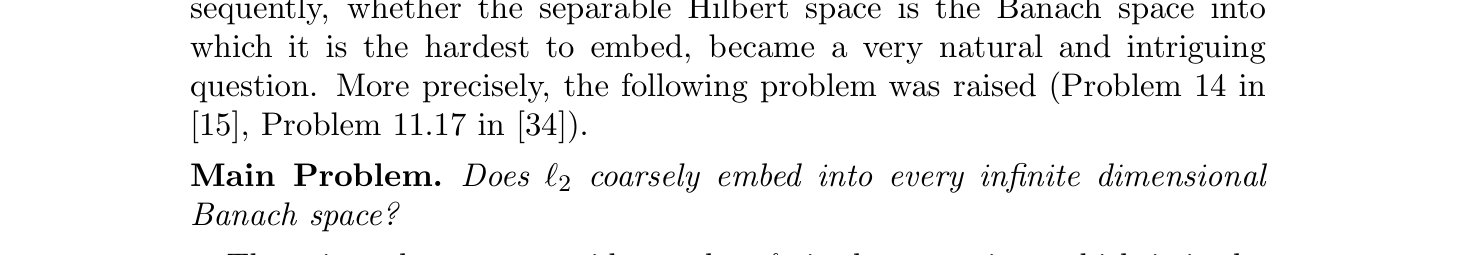
\includegraphics[width=\linewidth]{figures/supporting_restatement_crop.png}
\end{center}

The same paper then defines a Banach space to be coarsely minimal when it
coarsely embeds into every infinite-dimensional Banach space and records the
negative conclusion.

\begin{center}

\includegraphics[width=\linewidth]{figures/supporting_answer_crop.png}
\end{center}

\section*{Idea of the Proof}

The identification is direct rather than inferential. The source asks whether
\(\ell_2\) is universal for coarse embeddability into all infinite-dimensional
Banach spaces. Baudier--Lancien--Schlumprecht cite that exact problem, call such
universal spaces ``coarsely minimal'', and prove that no infinite-dimensional
Banach space is coarsely minimal. Their argument uses Tsirelson's original
space \(T^*\): a concentration inequality for infinite Hamming graphs in
\(T^*\) obstructs coarse embeddings of spaces whose spreading-model or metric
cotype structure is incompatible with \(T^*\). In particular, \(\ell_2\) fails
to coarsely embed into \(T^*\).

\section*{Formal Statement}

\begin{theorem}
Problem 14 of Godefroy--Lancien--Zizler, arXiv:1207.2958, has a negative
answer in the later literature. The Hilbert space \(\ell_2\) does not coarsely
embed into every infinite-dimensional Banach space.
\end{theorem}

\begin{proof}
Baudier--Lancien--Schlumprecht state that the question whether \(\ell_2\)
coarsely embeds into every infinite-dimensional Banach space was raised as
Problem 14 in \cite{GLZ2014}. This is the same question as the source Problem
14 displayed above.

Their Corollary B says that, for every \(p\in[1,\infty)\), the space
\(\ell_p\) does not coarsely embed into Tsirelson's original space \(T^*\).
Taking \(p=2\), \(\ell_2\) does not coarsely embed into \(T^*\). Since \(T^*\)
is an infinite-dimensional Banach space, this gives a negative answer to the
source question. Equivalently, their Corollary C states the stronger conclusion
that there is no coarsely minimal infinite-dimensional Banach space.
\end{proof}

\section*{Verification and Limitations}

The source PDF is stored as \texttt{source\_paper.pdf}. The supporting answer
PDF is stored as
\[
\texttt{supporting\_paper\_1705.06797.pdf}.
\]
The crops above come from page 33 of the source PDF and pages 2 and 4 of the
supporting PDF.

This packet does not answer the later final question in \cite{BLS2017} asking
whether \(\ell_2\) coarsely embeds into every super-reflexive Banach space. It
also does not use the run's human-only archive for the previously rejected
finite-dimensional literal reading of that later question.

Search bounds: before packaging, the run's registry, solutions index, attempts
index, and proof-gaps index were searched for arXiv:1207.2958, Problem 14,
coarsely minimal, and the \(\ell_2\)/every infinite-dimensional Banach-space
wording. A web/arXiv phrase search for the exact question found
arXiv:1705.06797, and its local TeX source was checked for the explicit
Problem 14 citation and negative conclusion.

\section*{References}

\begin{thebibliography}{9}

\bibitem{GLZ2014}
G. Godefroy, G. Lancien, and V. Zizler,
\emph{The non-linear geometry of Banach spaces after Nigel Kalton},
Rocky Mountain J. Math. 44 (2014), no. 5, 1529--1583.
arXiv:1207.2958.
\url{https://arxiv.org/abs/1207.2958}

\bibitem{BLS2017}
F. Baudier, G. Lancien, and Th. Schlumprecht,
\emph{The coarse geometry of Tsirelson's space and applications},
J. Amer. Math. Soc. 31 (2018), no. 3, 699--717.
arXiv:1705.06797.
\url{https://arxiv.org/abs/1705.06797}

\end{thebibliography}

\end{document}
